In Tabelle \ref{tab:info} sind die Literaturwerte zu den hier verwendeten
Elementen einzusehen. Die Glanzwinkel $\Theta$ berechnen sich nach Formel
\eqref{eqn:bragg} mit $E=h\cdot c / \lambda$.
\begin{table}[h]
  \centering
  \begin{tabular}{c c c c c}
    \toprule
    $\su{Metall}$  & $\su{Ordnungszahl} \,\, \su{Z}$ &
    $E^\su{Lit}_\su{K} \,/\, \keV$ & $\theta^\su{Lit}_\su{K}\,/\,\si{\degree}$ & $\sigma_\su{K}$ \\
    \midrule
     Zn & 30 & 9.65 & 18.6 & 3.56 \\
     Ge & 32 & 11.11 & 16.1 & 3.66 \\
     Br & 35 & 13.47 & 13.2 & 3.85 \\
     Sr & 38 & 16.10 & 11.0 & 4.00 \\
     Zr & 40 & 17.09 & 9.0 &  5.04 \\
     Au & 79 & 13.70 & 13.0 (LII) &  \hrulefill\\
     Au & 79 & 11.92 & 15.0 (LIII) & \hrulefill \\
    \bottomrule
  \end{tabular}
  \caption{Literaturwerte der Metalle \cite{Elit},\,\cite{KAu}}
  \label{tab:info}
\end{table}
Zu Beginn wird die Bragg-Bedingung überprüft. Der Graph in Abbildung \ref{fig:Bragg3}
lässt einen Glanzwinkel von ca. $2\Theta = 26.8 \,\si{\degree}$ erkennen.
\begin{figure}
  \centering
  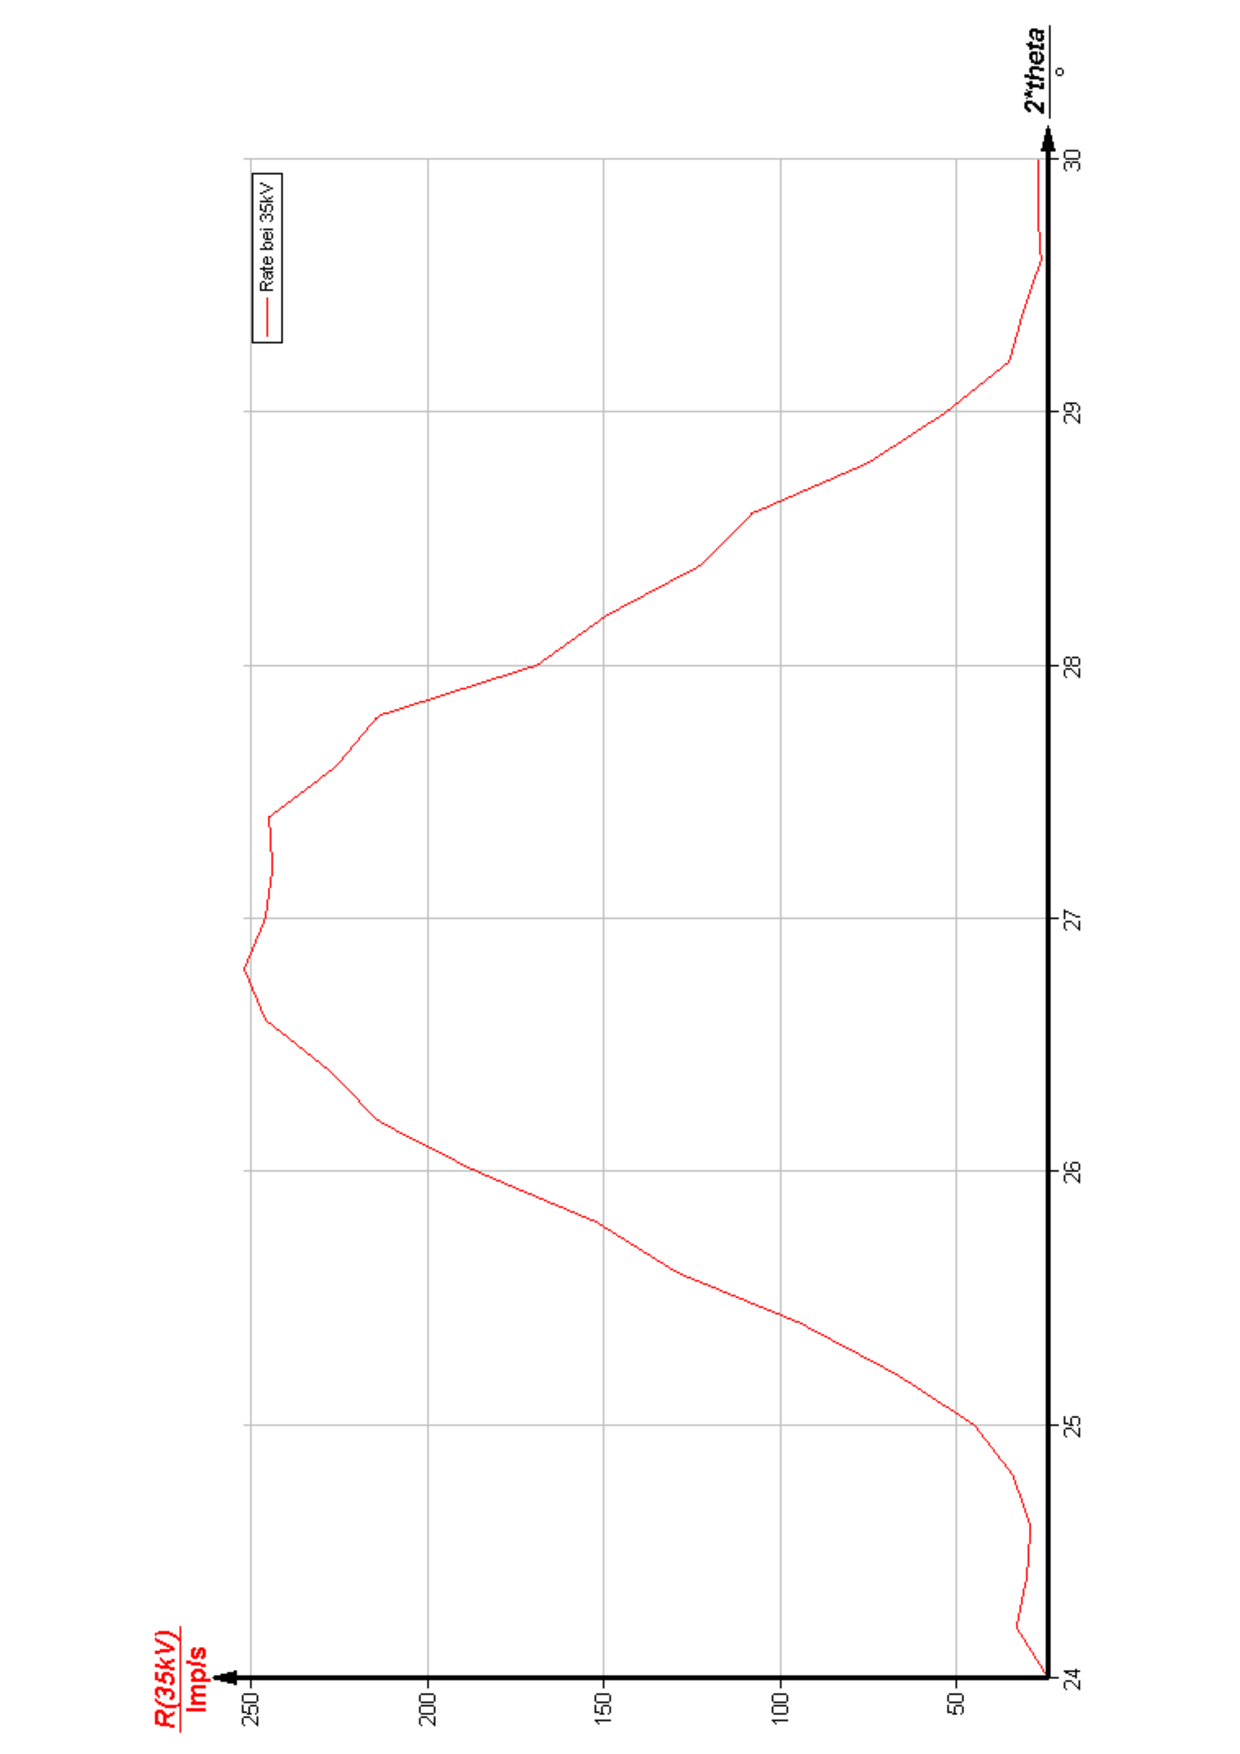
\includegraphics[width=0.5\textwidth, angle=270]{bilder/Bragg3.pdf}
  \caption{Überprüfung der Bragg-Bedingung.}
  \label{fig:Bragg3}
\end{figure}
Dies stimmt mit
dem eingestellten Kristallwinkel von $\Theta = 14\,\si{\degree}$ ungefähr überein,
wodurch die Bragg-Bedingung bestätigt wird.

Anschließend wird das Emissionssprektrum der Cu-Röntgenröhre untersucht.
Dieses Spektrum ist in Abb. \ref{fig:EmissionCu} zu sehen.
\begin{figure}[h]
  \centering
  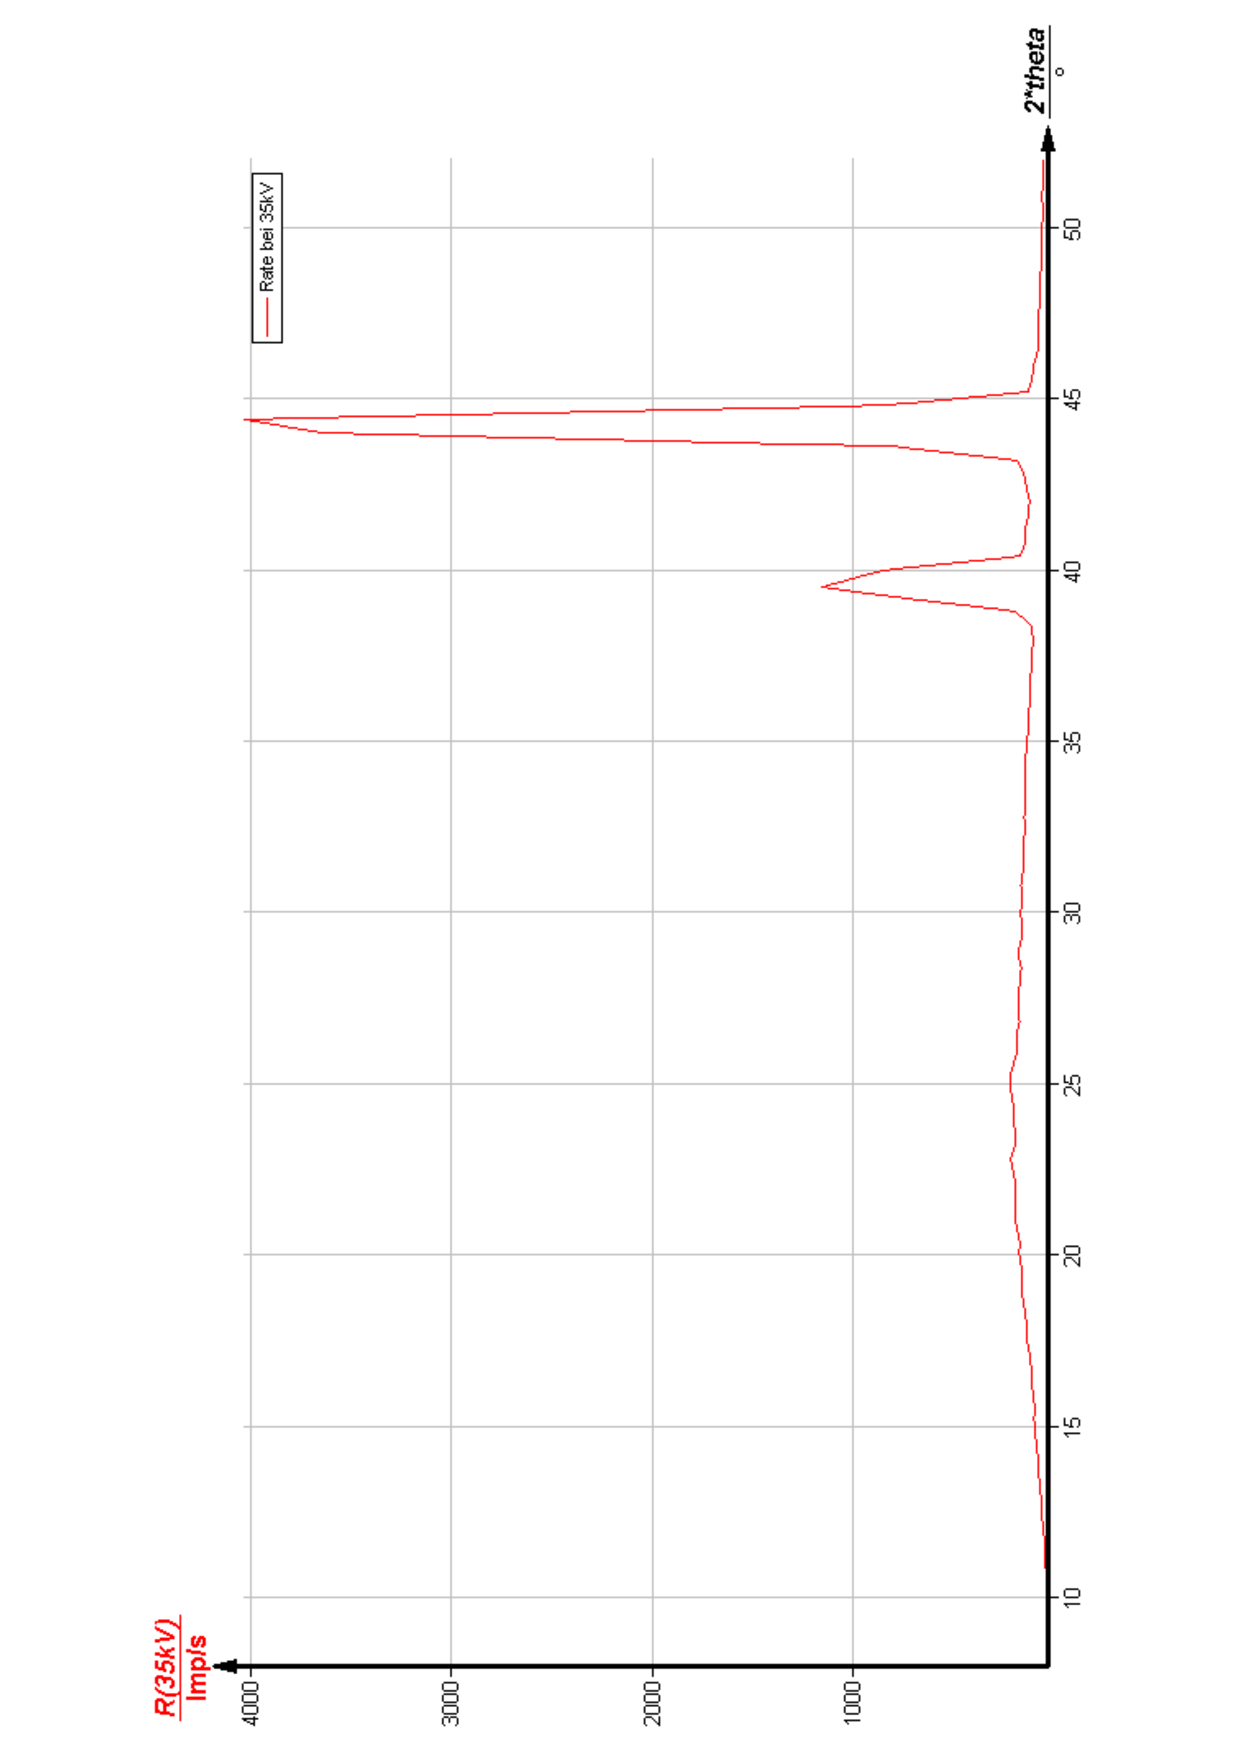
\includegraphics[width=0.5\textwidth, angle=270]{bilder/EmissionCu.pdf}
  \caption{Emissionspektrum der Cu-Röntgenröhre.}
  \label{fig:EmissionCu}
\end{figure}
Der vordere Peak steht für die $K_\su{\beta}$ und der hintere für die $K_\su{\alpha}$
Linie. Die Halbwertsbreite, bei der die Intensität auf die Hälfte abgesunken ist,
der $\beta$-Linie läuft von $\Theta = 19.5\,\si{\degree}$ bis $\Theta = 20.1\dgr$.
Die der $\alpha$-Linie läuft von $\Theta = 21.9\dgr$ bis $\Theta = 22.3\dgr$.
Die Energien ergeben sich damit zu
\begin{align}
  E_\su{\Theta_1, \beta} &= 10.23 \keV \\
  E_\su{\Theta_2, \beta} &= 9.93 \keV \\
  E_\su{\Theta_1, \alpha} &= 9.14 \keV \\
  E_\su{\Theta_2, \alpha} &= 8.00 \keV. \\
\end{align}
Das Auflösungsvermögen berechnet sich durch die Differenz der jeweiligen Energien,
also
\begin{equation}
  \Delta E = E_2 - E_1.
\end{equation}
Damit folgt
\begin{align}
  \Delta E_\su{\alpha} &= 0.30 \keV  \\
  \Delta E_\su{\beta} &= 0.15 \keV. \\
\end{align}

Die maximale Energie lässt sich auch über \eqref{eqn:bragg} bestimmen. Für $\Theta$
wählt man dazu den Grenzwinkel, also den Winkel, bei dem das Sprektrum beginnt.
Somit gilt
\begin{equation}
  \Theta = 8.0 \dgr.
\end{equation}
Damit ergibt sich eine Energie von
\begin{equation}
  E_\su{max} = 24.61 \keV.
\end{equation}
Aus der Umstellung
\begin{equation}
  \lambda = \frac{hc}{E}
\end{equation}
ergibt sich eine Wellenlänge von $\lambda=5.04\,\cdot10^{-8}\nm$
Nun werden die Aktivierungsenergien und die Abschirmkonstanten
der verschiedenen Elemente untersucht. Die
Werte sind in Tabelle \ref{tab:Energie} einzusehen. Die Abschirmkonstanten $\sigma_\su{K}$
lassen sich mittels \eqref{eqn:abschirmK} berechnen.
\begin{table}
  \centering
  \begin{tabular}{c c c c}
    \toprule
    $\su{Element}$ & $\Theta_\su{abgelesen} \,/\dgr$ & $E_\su{K_\su{\alpha}}\,/ \keV$ & $\su{Abschirmkonstante}\,\,\sigma_\su{K}$\\
    \midrule
    Zn & 19.90 &  9.06 & 4.39   \\
    Ge & 16.00 & 11.18 & 3.56   \\
    Br & 13.15 & 13.56 & 3.74   \\
    Sr & 10.85 & 16.38 & 3.69   \\
    Zr & 10.75 & 16.46 & 5.70   \\
    \bottomrule
  \end{tabular}
  \caption{Aktivierungsenergien und Abschirmkonstanten der einzelnen Elemente.}
  \label{tab:Energie}
\end{table}
Die Abschirmkonstante $\sigma_\su{L}$
von Gold lässt sich mittels \eqref{eqn:abschirmL} bestimmen.
Für die $LII$ Kante wird der Winkel $\Theta_\su{exp,1} = 12.7 \dgr$ und für die $LIII$ Kante
wird der Winkel $\Theta_\su{exp,2} = 14.9 \dgr$ verwendet. Die theoretischen Winkel lauten
$\Theta_\su{theo,1} = 13.0 \dgr$ und $\Theta_\su{theo,2} = 15.0 \dgr$.
Die Energien ergeben sich wieder mittels \eqref{eqn:bragg}. Daraus wird
\begin{align*}
  \Delta E &= E_\su{LII} - E_\su{LIII} \\
  \Delta E_\su{theo} &= 1.78 \keV \\
  \Delta E_\su{exp} &= 2.03 \keV \\
\end{align*}
bestimmt.
Damit ergeben sich folgende Abschirmkonstanten:
\begin{align*}
  \sigma_\su{L, theo} &= 3.91  \\
  \sigma_\su{L, exp} &= 1.70 \\
\end{align*}

Nachfolgend sind alle gemessenen Spektren zu sehen. Dabei zeigt Abb. \ref{fig:Zink}
das Spektrum zu Zink, Abb. \ref{fig:Germanium} zeigt Germanium, Abb. \ref{fig:Brom}
zeigt Brom, Abb. \ref{fig:Strontium} zeigt Strontium und Abb. \ref{fig:Zirkonium} zeigt
Zirkonium. Abb. \ref{fig:Aurum} zeigt Gold.
\begin{figure}
  \centering
  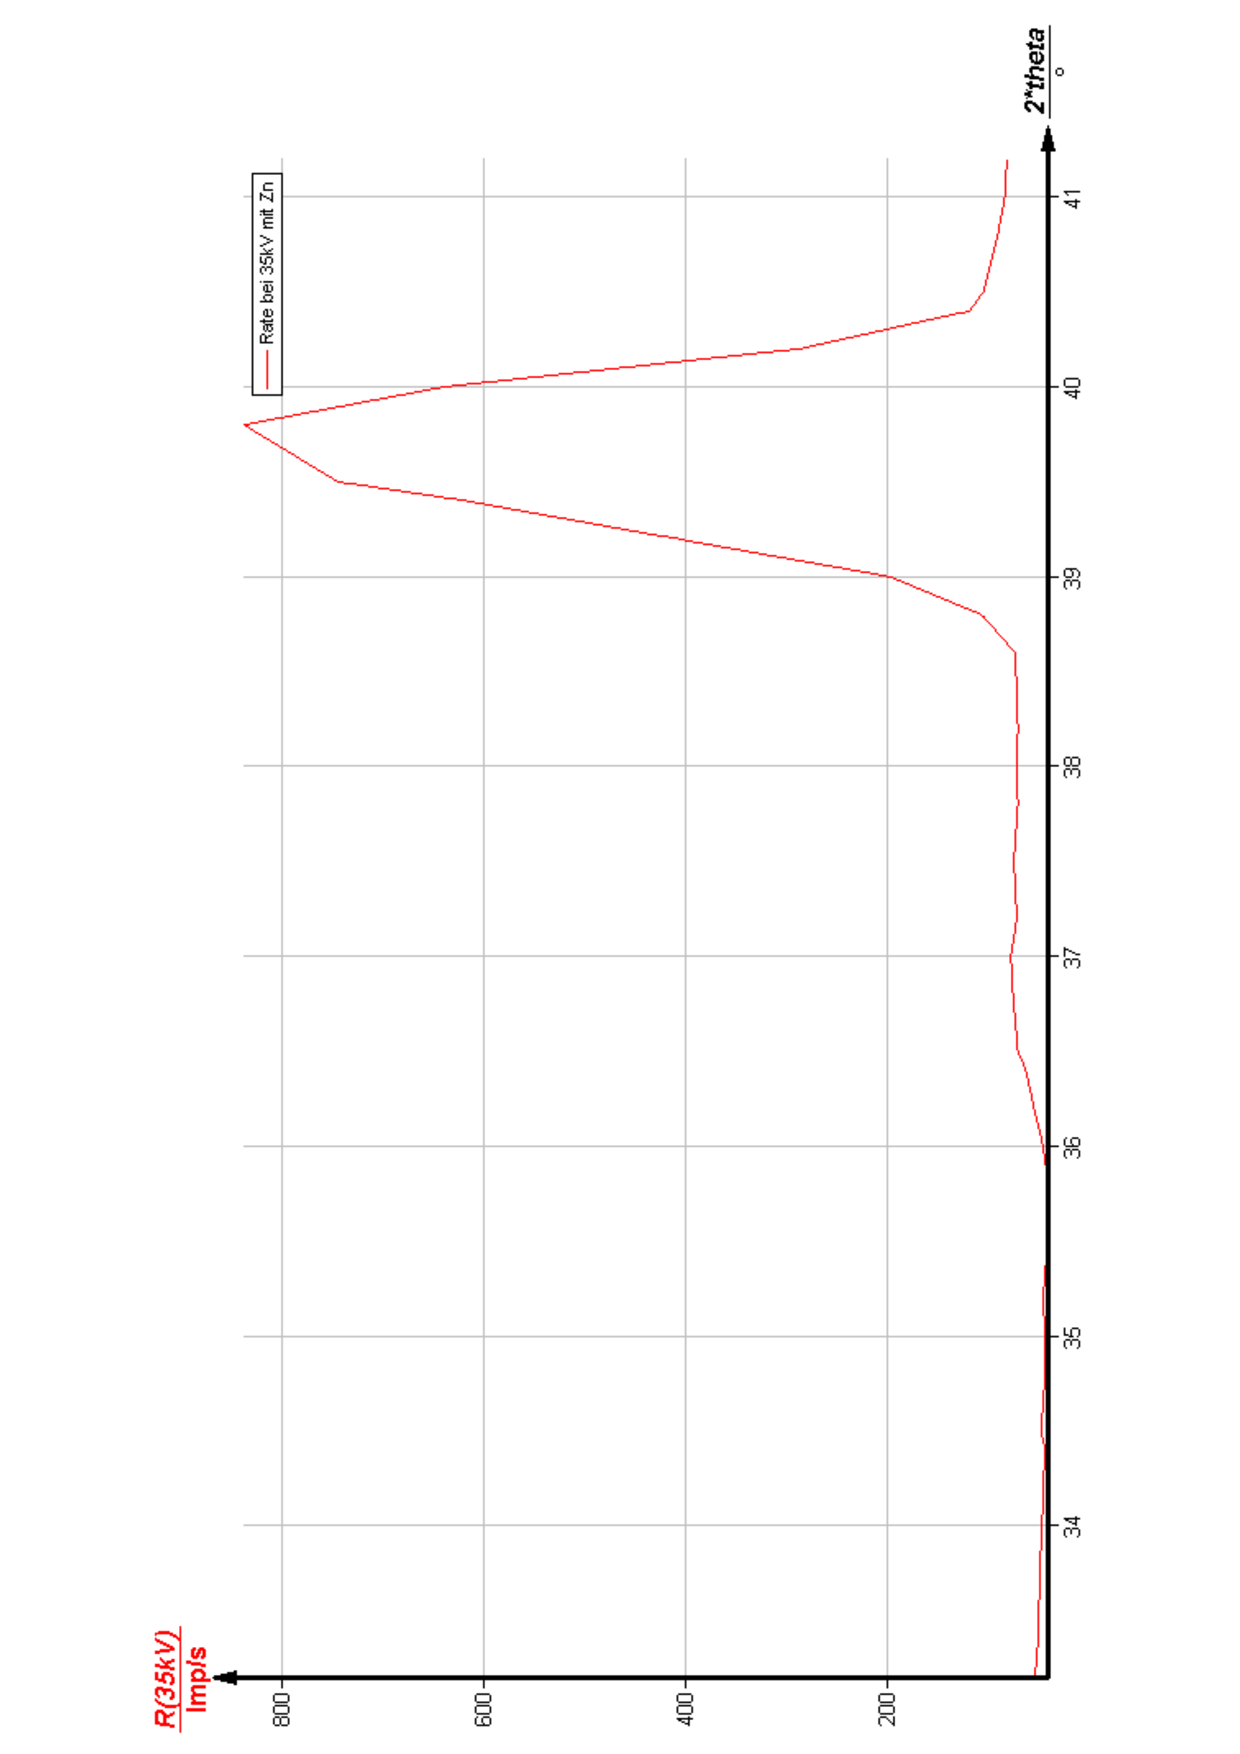
\includegraphics[width=0.5\textwidth, angle=270]{bilder/AbsorpZn.pdf}
  \caption{Absorptionsspektrum von Zink.}
  \label{fig:Zink}
\end{figure}
\begin{figure}
  \centering
  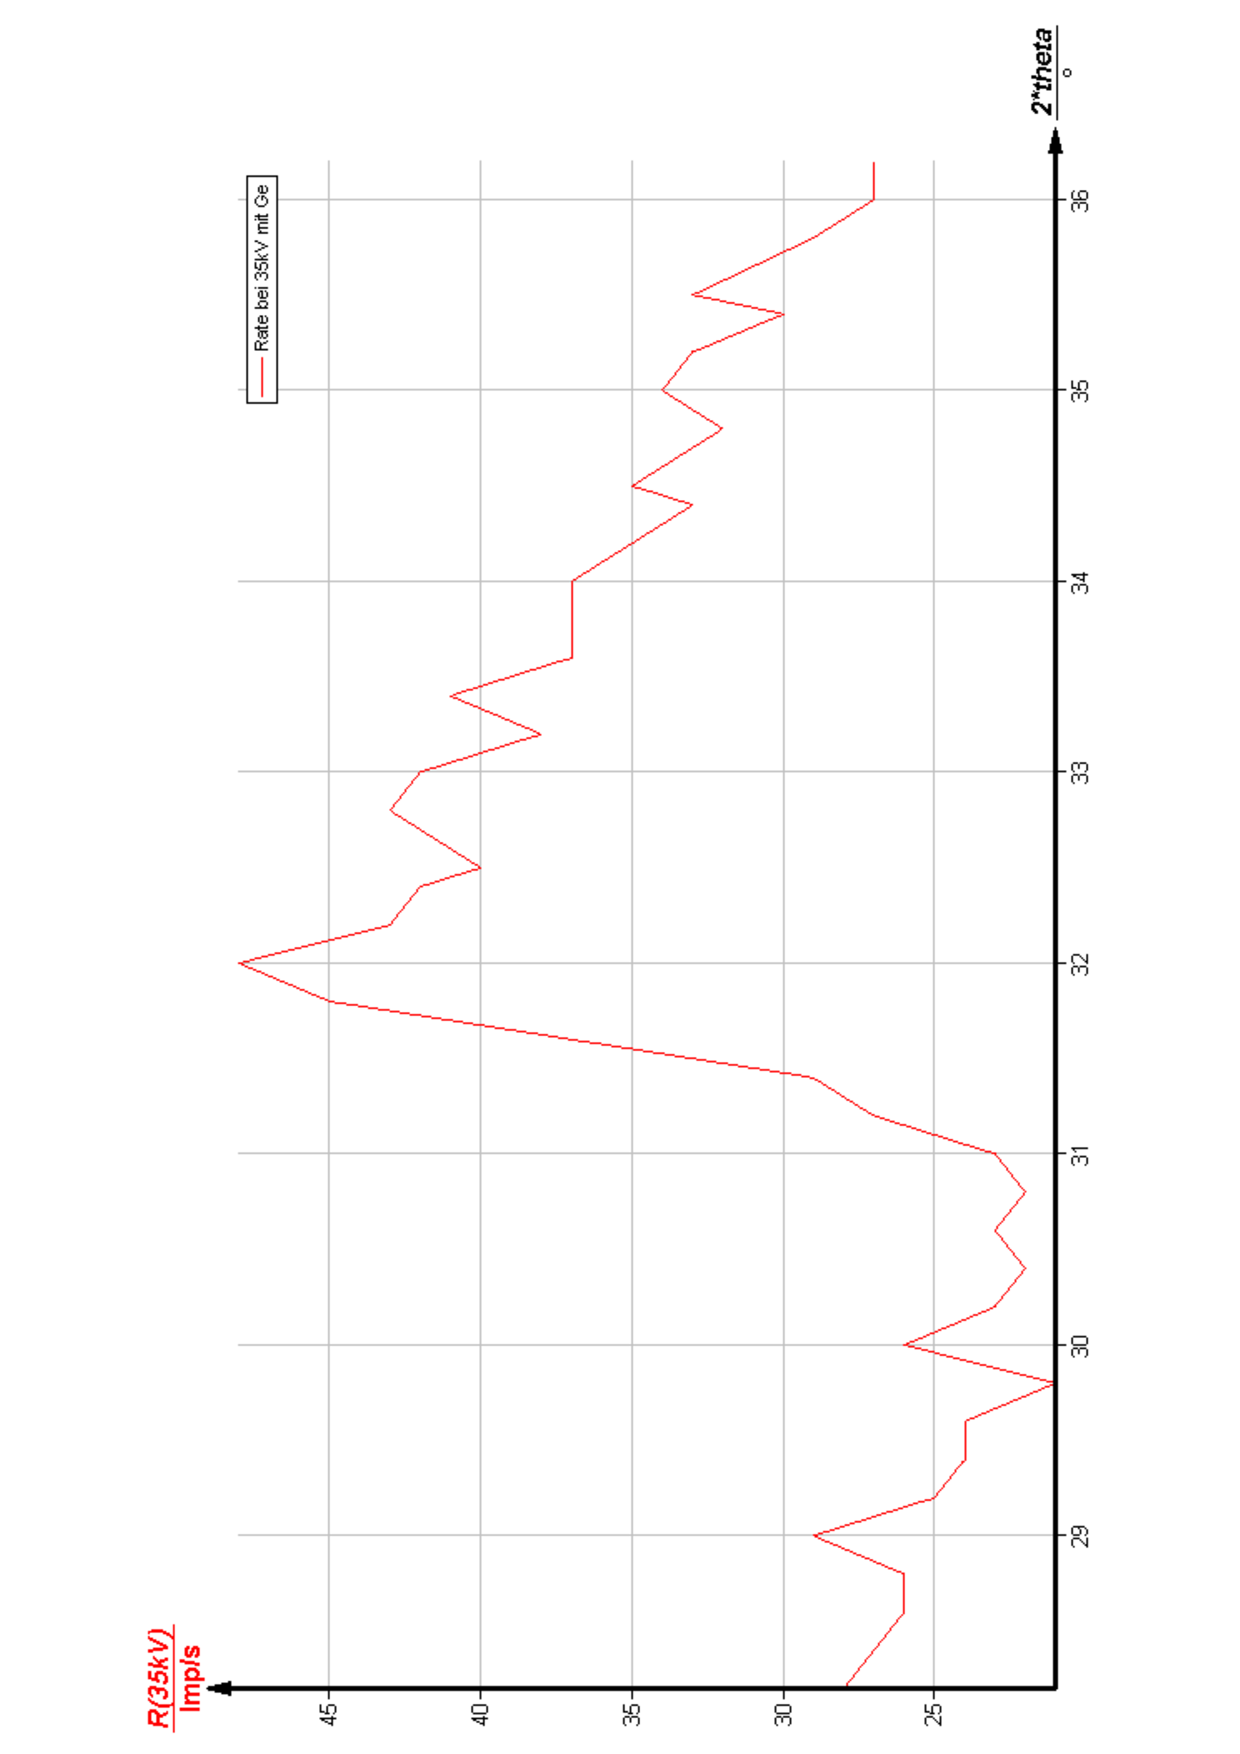
\includegraphics[width=0.5\textwidth, angle=270]{bilder/AbsorpGe.pdf}
  \caption{Absorptionsspektrum von Germanium.}
  \label{fig:Germanium}
\end{figure}
\begin{figure}
  \centering
  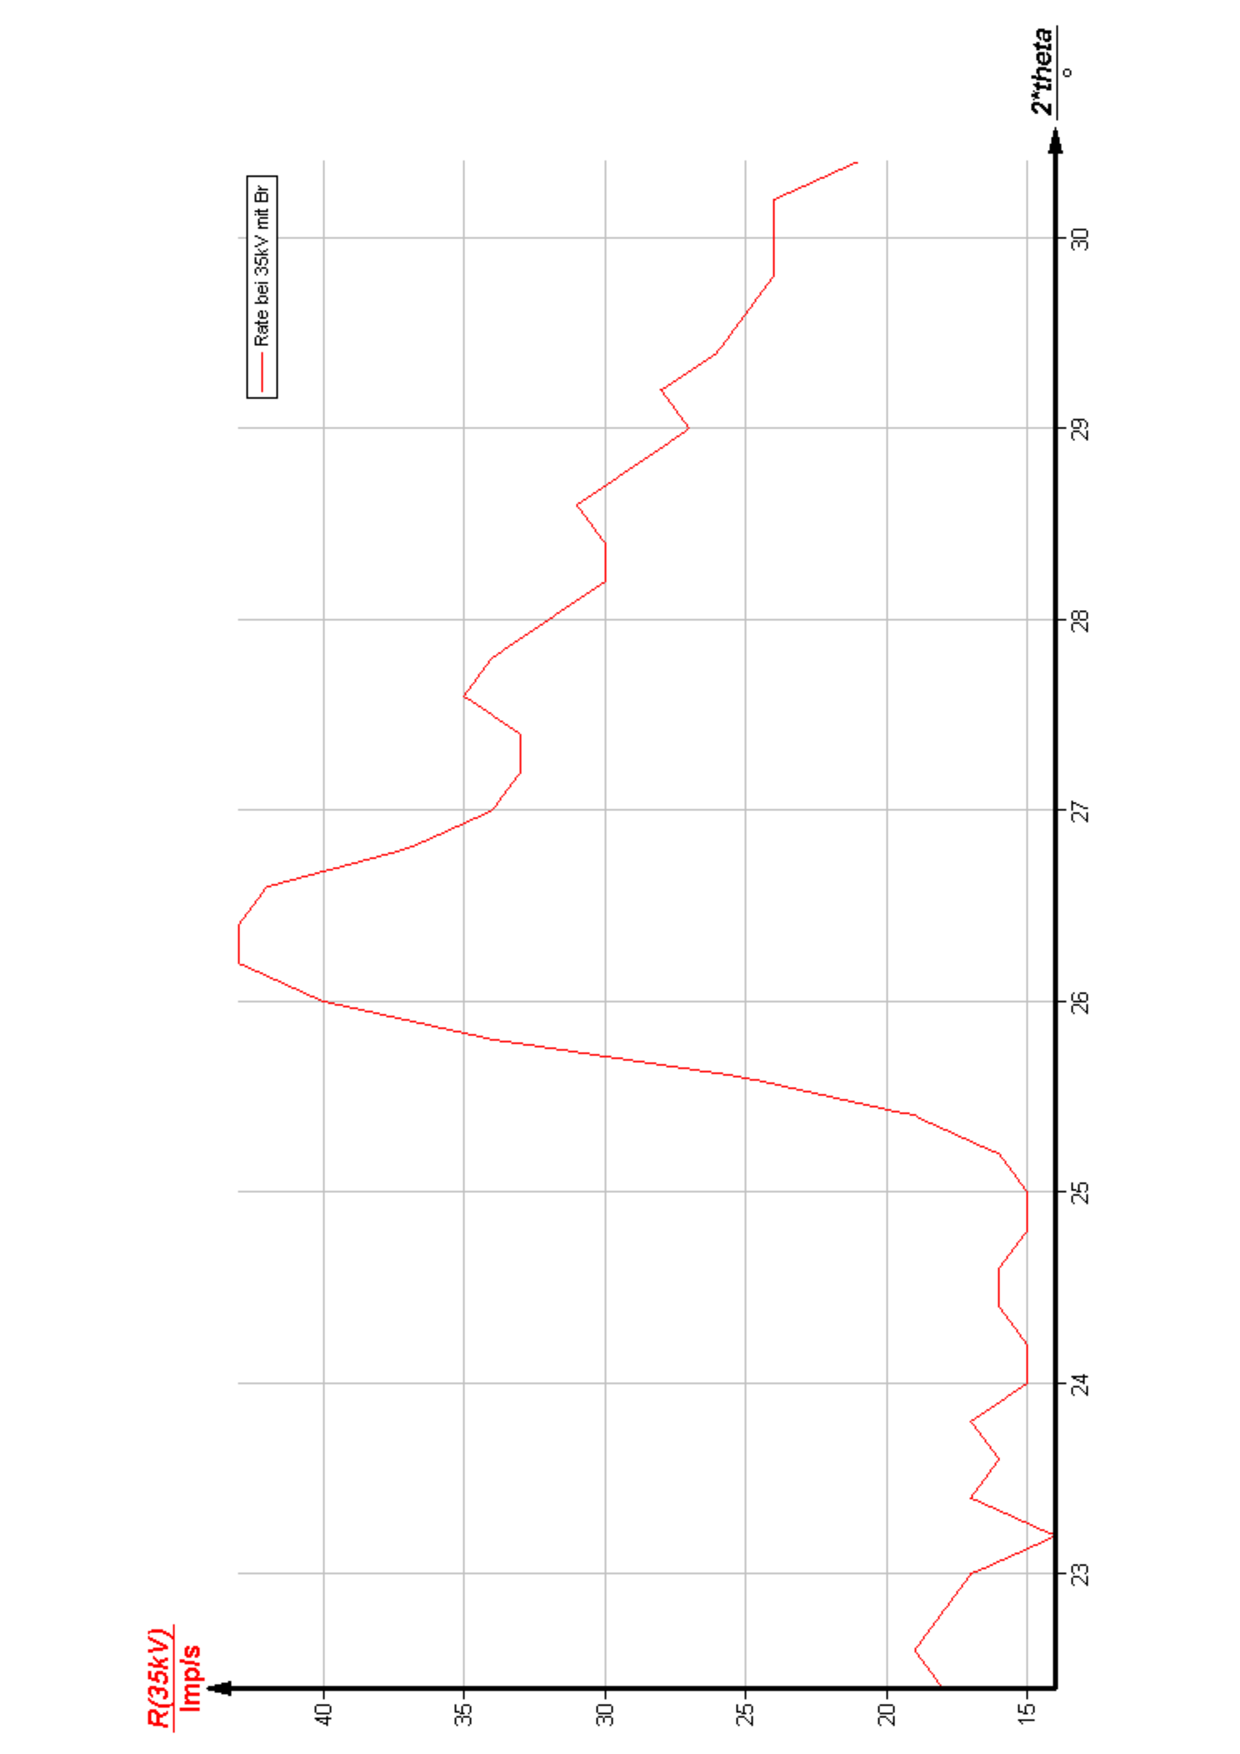
\includegraphics[width=0.5\textwidth, angle=270]{bilder/AbsorpBr.pdf}
  \caption{Absorptionsspektrum von Brom.}
  \label{fig:Brom}
\end{figure}
\begin{figure}
  \centering
  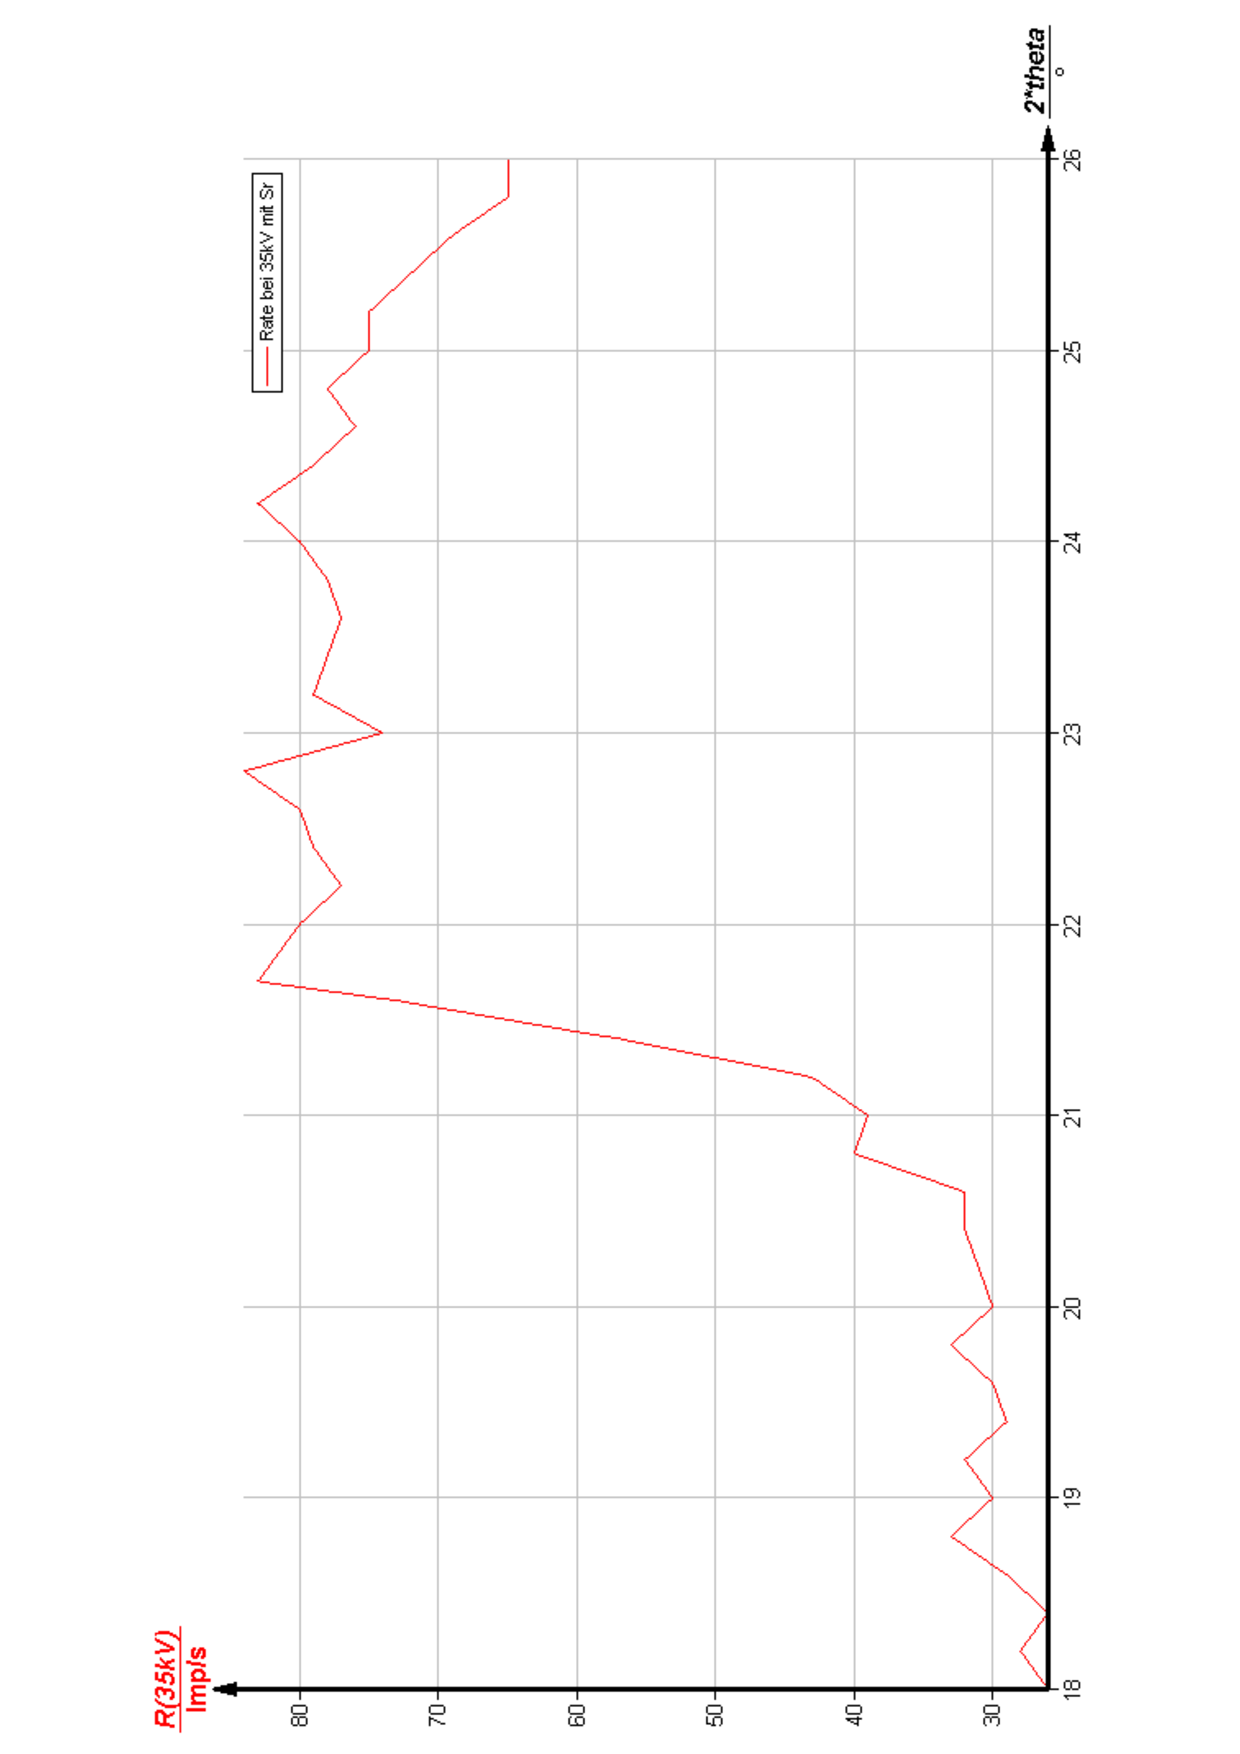
\includegraphics[width=0.5\textwidth, angle=270]{bilder/AbsorpSr.pdf}
  \caption{Absorptionsspektrum von Strontium.}
  \label{fig:Strontium}
\end{figure}
\begin{figure}
  \centering
  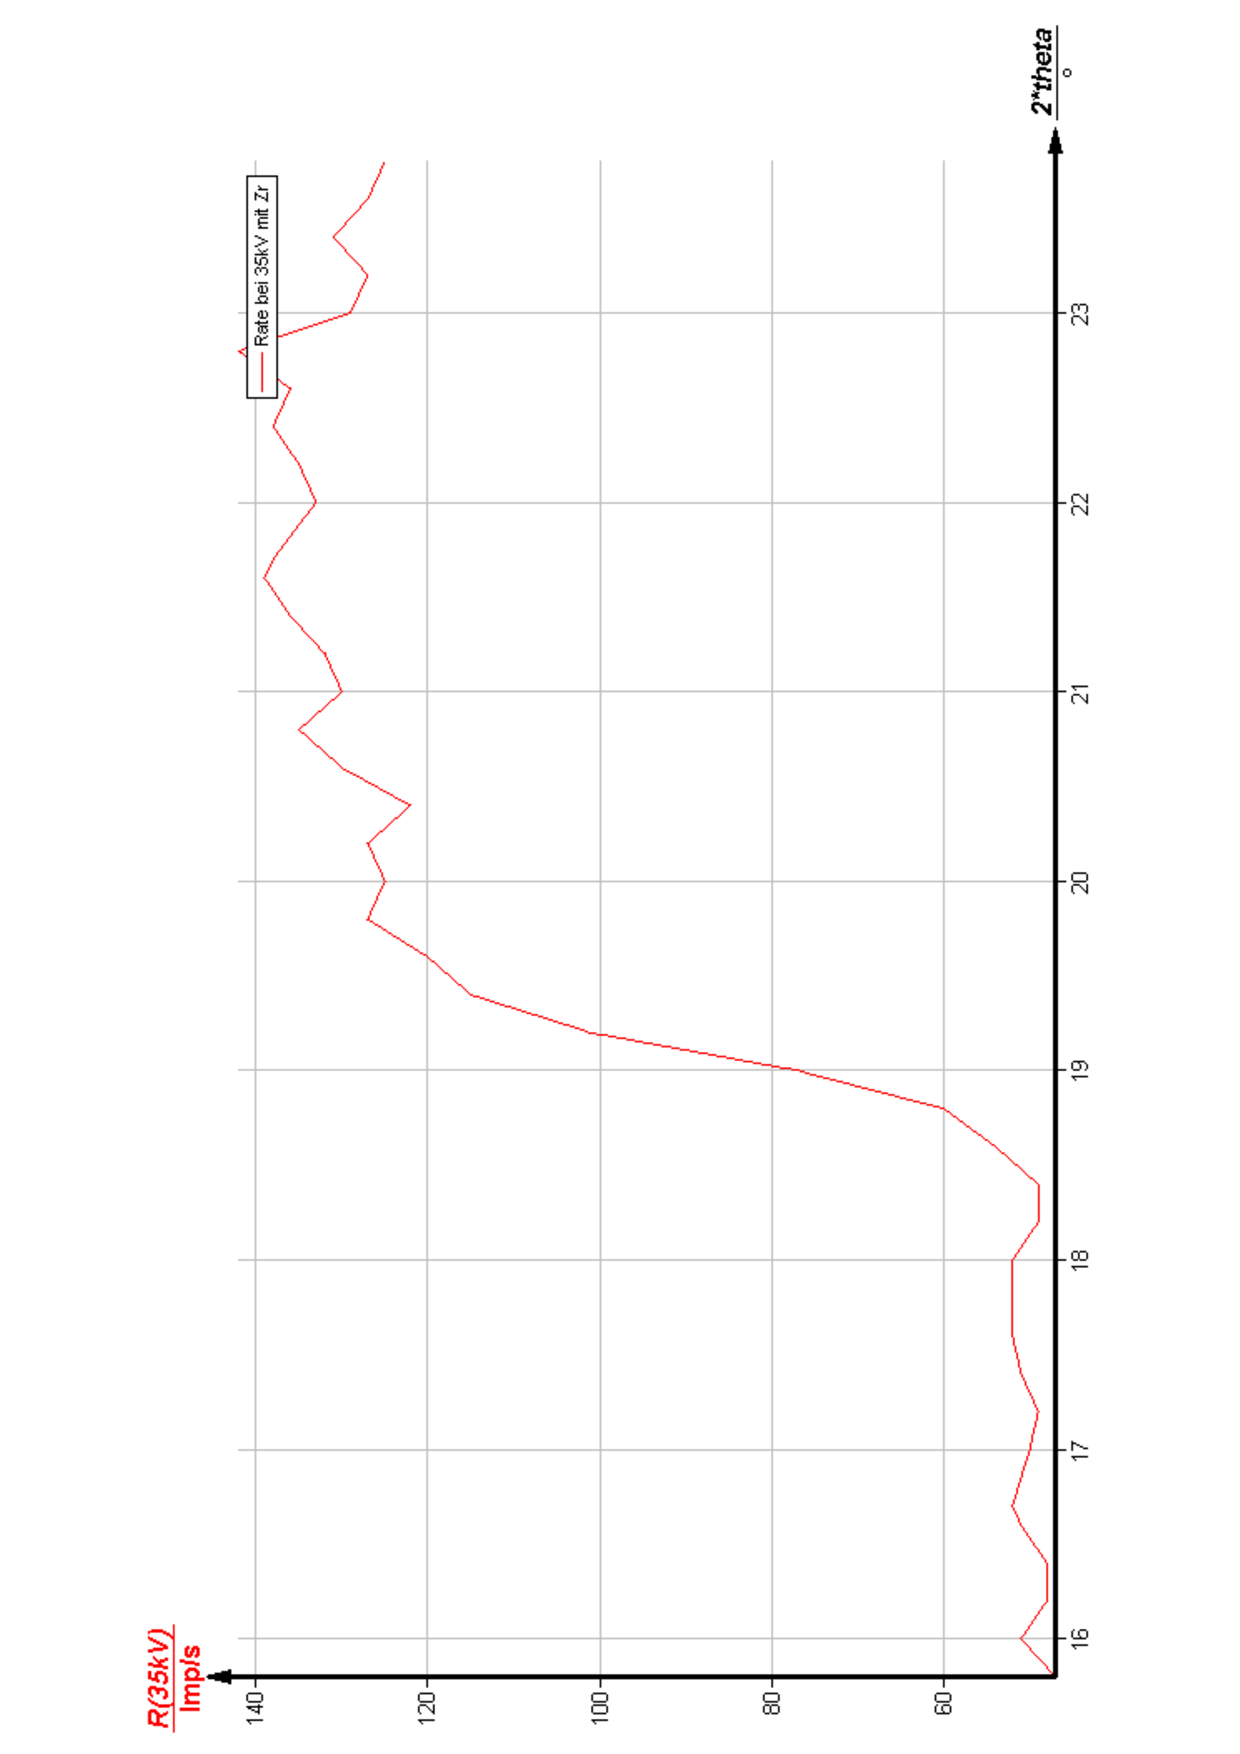
\includegraphics[width=0.5\textwidth, angle=270]{bilder/AbsorpZr.pdf}
  \caption{Absorptionsspektrum von Zirkonium.}
  \label{fig:Zirkonium}
\end{figure}
\begin{figure}
  \centering
  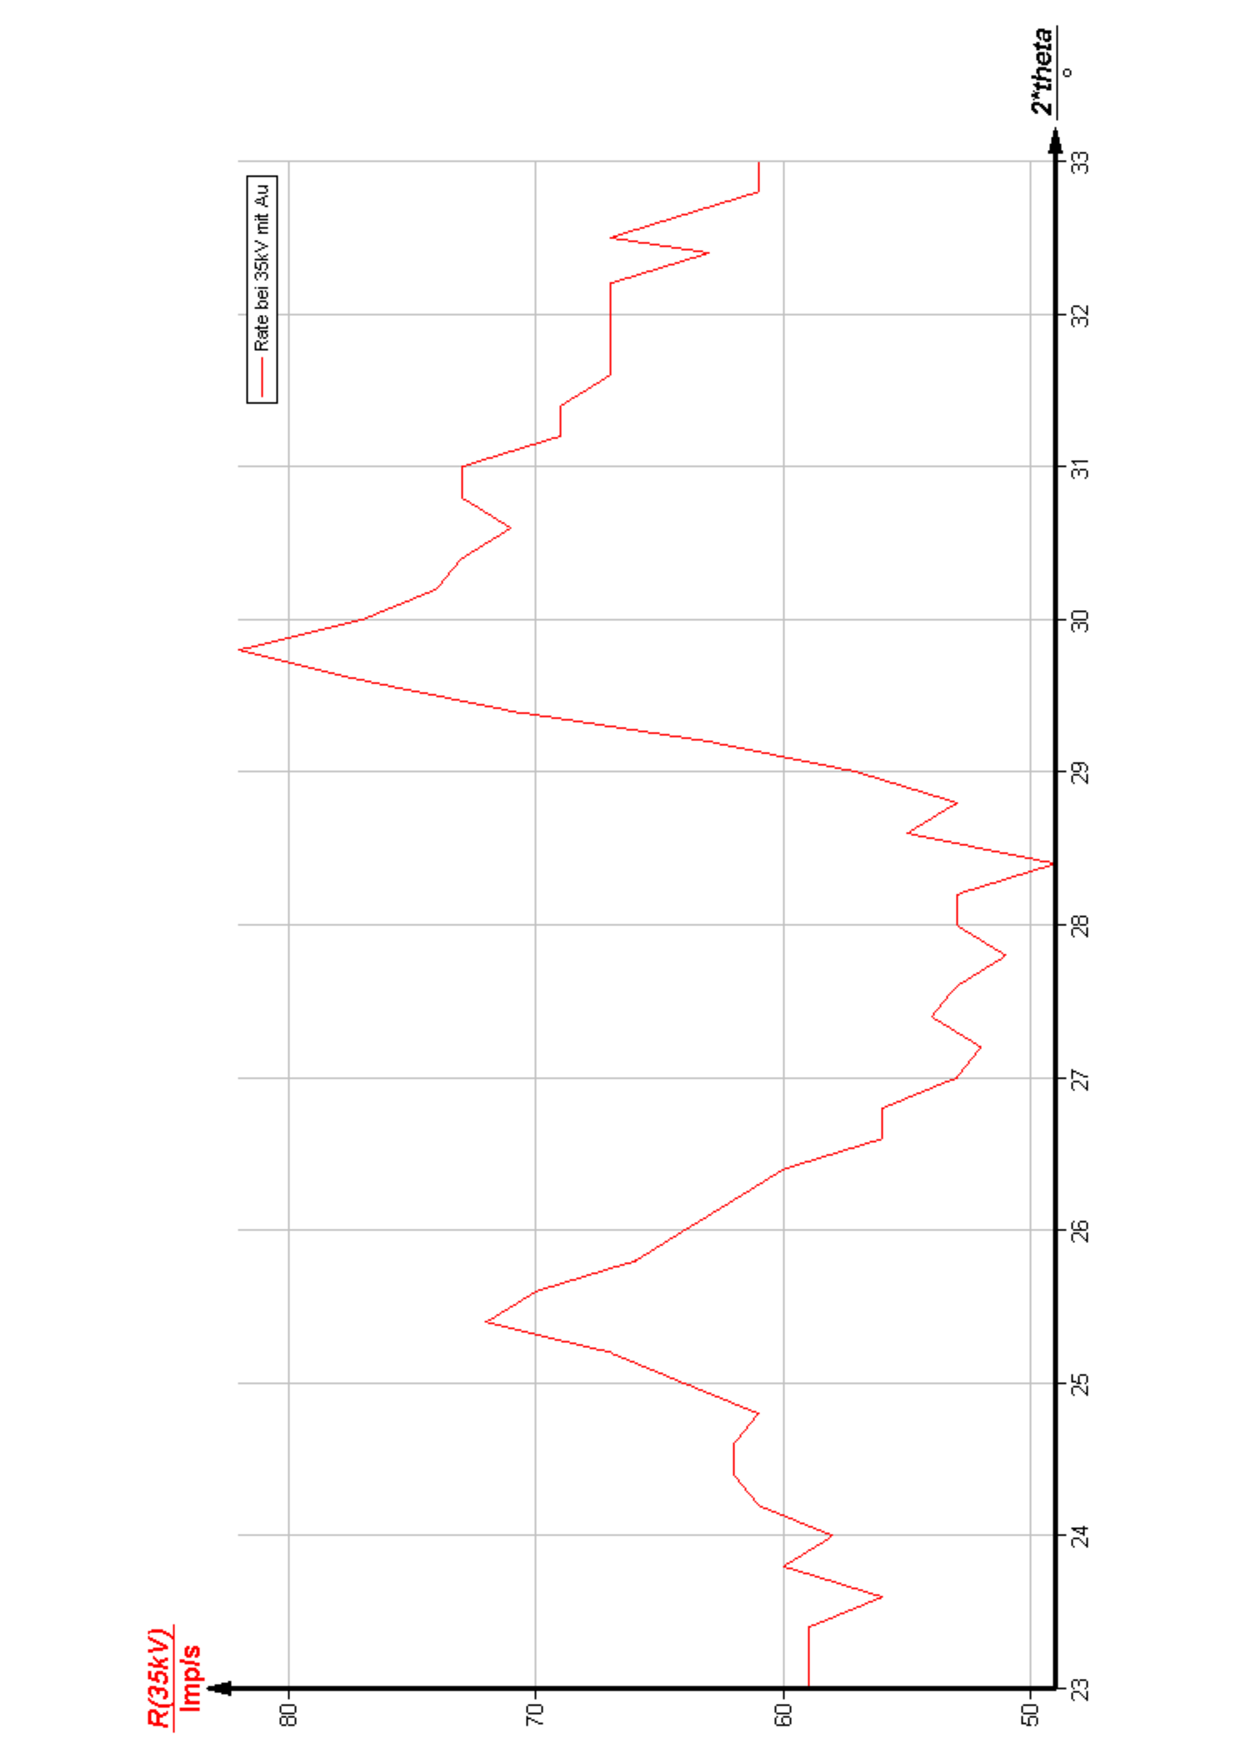
\includegraphics[width=0.5\textwidth, angle=270]{bilder/AbsorpAu.pdf}
  \caption{Absorptionsspektrum von Aurum.}
  \label{fig:Aurum}
\end{figure}

\newpage
Nun wird Moseley's Gesetzt überprüft. Dazu wird $\sqrt{E_K}$ gegen $Z^2$ aufgetragen.
Der Graph ist in Abb. \ref{fig:Mose} zu sehen.
Dabei ergeben sich die Parameter:
\begin{align*}
  a &= (22 \pm 4) \,1\,/\, \sqrt{\si{\electronvolt}}\\
  b &= (-1300 \pm 400). \\
\end{align*}
\begin{figure}[h]
  \centering
  \includegraphics[width= 8cm]{bilder/plot.pdf}
  \caption{Lineare Ausgleichsrechnung zu Überprüfung des Moseleyschen Gesetzes.}
  \label{fig:Mose}
\end{figure}
Die Steigung $a$ entspricht der Rydberg-Energie.
Über den Zusammenhang
\begin{equation*}
  E_\su{R}=hcR_\infty
\end{equation*}
erhält man für die Rydberg-Konstante $R_\infty$ einen Wert von
\begin{equation*}
  R_\infty=1.8\,\cdot10^7 \mt^{⁻1}
\end{equation*}
